\documentclass{scrreprt}
\usepackage{array}
\usepackage{graphicx}
\usepackage{listings}
\usepackage{underscore}
\usepackage[bookmarks=true]{hyperref}
\usepackage[utf8]{inputenc}
\usepackage{float}
\usepackage[french]{babel}
\hypersetup{
    bookmarks=false,    % show bookmarks bar
    pdftitle={rapport_conception_Lambolez_Petit},    % title
    pdfauthor={Théodore Lambolez, Maximilien Petit},                     % author
    pdfsubject={TeX and LaTeX},                        % subject of the document
    pdfkeywords={TeX, LaTeX, graphics, images}, % list of keywords
    colorlinks=true,       % false: boxed links; true: colored links
    linkcolor=blue,       % color of internal links
    citecolor=black,       % color of links to bibliography
    filecolor=black,        % color of file links
    urlcolor=black,        % color of external links
    linktoc=page            % only page is linked
}
\def\myversion{1.0}
\date{}
%\title
\usepackage{hyperref}
\begin{document}
\begin{figure}
   \begin{minipage}[c]{.46\linewidth}
      
\includegraphics[scale=0.3]{images/telecom.png}
   \end{minipage} \hfill
   \begin{minipage}[c]{.46\linewidth}
      
\includegraphics[scale=1.9]{images/lorraine.jpg}
   \end{minipage}
\end{figure}
\begin{flushright}
    \rule{15cm}{5pt}
    \vskip1cm
\end{flushright}
\begin{center}
	\vspace{3cm}
	\fbox{
	\begin{minipage}{0.9\textwidth}
        	\Huge{
			\textbf{
			\begin{center}
				Projet de conception : \\
				Gestion des Stages
				\vspace{0.5cm}
			\end{center}
			}
		}
	\end{minipage}
	}
\end{center}
\begin{flushright}
        \vspace{5cm}
	\huge{
        \textbf{
	Ecrit par \\
	\vspace{0,875cm}
	\href{mailto:theodore.lambolez@telecomnancy.eu}{Théodore Lambolez} \\
	\href{mailto:maximilien.petit@telecomnancy.eu}{Maximilien Petit}\\
	}
	}
        \vspace{0,5cm}
        \large{
	\textbf{
	\today\\
	}	
	}
\end{flushright}

\tableofcontents

\chapter{Introduction}
%\addcontentsline{toc}{chapter}{Introduction}

Ce devoir de conception permet l'approfondissement du travail déjà réalisé lors du 
cahier des charges. Cette partie a pour but de rendre plus efficace et plus réfléchie la phase 
de développement du logiciel. Ici, nous ne nous intéresserons pas à tous les cas d'utilisation 
de la gestion des stages mais seulement à certains d'entre eux dans le but de nous exercer. Ainsi, 
nous détaillerons à l'aide de diagrammes UML le système de saisie de la fiche de renseignement, de  
validation de cette fiche ainsi que le système de passage d'une année à l'autre.  

	Pour ce faire, nous verrons d'abord le diagramme d'activité qui nous aidera à avoir une vision 
d'ensemble de la demande de stage jusqu'à la signature de la convention en passant par le remplissage
de la fiche de renseignement. Ensuite, nous approfondirons les trois diagrammes de séquences. Le diagramme
de classe placé en dernière partie pourra être utilisé comme annexe. 

\newpage
\chapter{Diagramme d'état}
%\addcontentsline{toc}{chapter}{Diagramme d'état}

	Nous commencerons ici par expliquer le diagramme d'état qui nous permettra d'avoir une meilleur vue d'ensemble
du processus de demande de stage jusqu'à la création de la convention signée par tous les partis concernés. 

	Tout d'abord, nous avons réalisé un état pour la création de la fiche de renseignement qui se fait en deux 
étapes. Deux états principaux sont donc à distinguer: un pour la fiche de renseignement côté élève et un autre pour 
la fiche de renseignement côté entreprise. Sachant qu'il y a nécessairement la partie élève avant 
la partie entreprise puisque parmi les informations données par l'élève, il y a le mail permettant au système de 
créer le compte de l'entreprise. On distingue dans la création de ces deux parties, la création pour la première fois et 
la modification des données. En effet, lors du processus de validation, un élève ou le référent en entreprise peut être 
amené à réaliser des modifications. 
	Une fois la fiche de renseignement réalisée, elle est passée en validation. Elle sera alors enregistrée sur la base
de données puis transmise à l'administration. 
	Une fois les données récupérées par l'administration, l'application tente de créer automatiquement à partir des données
et d'un template, la convention. Elle est vérifiée par l'administration qui choisira soit de recréer une autre convention manuellement
soit de la conserver. 
	Une fois validée, la convention temporaire est sauvegardée sur la base de données puis transmise aux personnes concernées les invitant
à apposer leur signature. 
	Une fois que toutes les signatures sont récupérées, le système récupère ces signatures par un sytème de traitement numérique de l'image 
(en supposant qu'on ait fait des cadres de signatures pour toutes les personnes concernées). De cette manière, on peut obtenir la convention contenant
toutes les signatures. Celle-ci remplacera la convention temporaire dans la base de données puis sera envoyée  aux intéressés.  


\newpage
\chapter{Diagramme de séquence}
%\addcontentsline{toc}{chapter}{Diagramme de séquence}

	Dans cette section, nous aborderons les trois diagrammes de séquences demandés : la saisie de la fiche de renseignement,
la validation de celle-ci par le professeur responsable du stage ainsi que la transition d'une année scolaire à une autre.

\newpage
\section{Cas de la saisie}

	Ce diagramme de séquence sera traité en deux diagrammes différents puisque notre choix de conception est d'avoir réalisé
la fiche de renseignement en deux saisies distinctes.

	Tout d'abord une fois qu'un étudiant aura rempli le formulaire de la première partie de la fiche de renseignement en ligne et aura
appuyé sur le bouton "soumettre les informations", la classe gérant l'interface graphique appellera sur le contrôleur la fonction 
submitStudentData(Data d). La dénomination "Data d" fait en fait ici référent à tous les renseignements que l'élève donne lors de 
cette saisie. Les plus importantes pour bien comprendre ici sont le nom de l'entreprise et le mail du futur référent du stage au sein
celle-ci. Suite à ceci, le contrôleur gère la suite. Il commencera par déterminer si l'entreprise existe déjà ou non. Dans le cas où
ce test s'avère être négatif, il créera lui-même une instance de la classe "Company" en remplissant les premières informations la 
concernant comme son nom. Ensuite, le contrôleur devra rechercher l'instance de la classe "Student" correspondant à l'étudiant qui
a effectué la saisie, de manière à ce que le contrôleur puisse créer une instance de la classe "InformationSheet" qui aura accès aux instances
de "Student" et de "Company" qui la concerne. Ce nouvel objet stage sera créé en initialisant certaines de ses données avec celles qui lui
auront été founies. De plus, cette instance de "InformationSheet" s'ajoutera aux instance de "Student" et "Company" correspondant pour finir 
d'effectuer le lien.

\newpage
\begin{figure}[h]
\centering
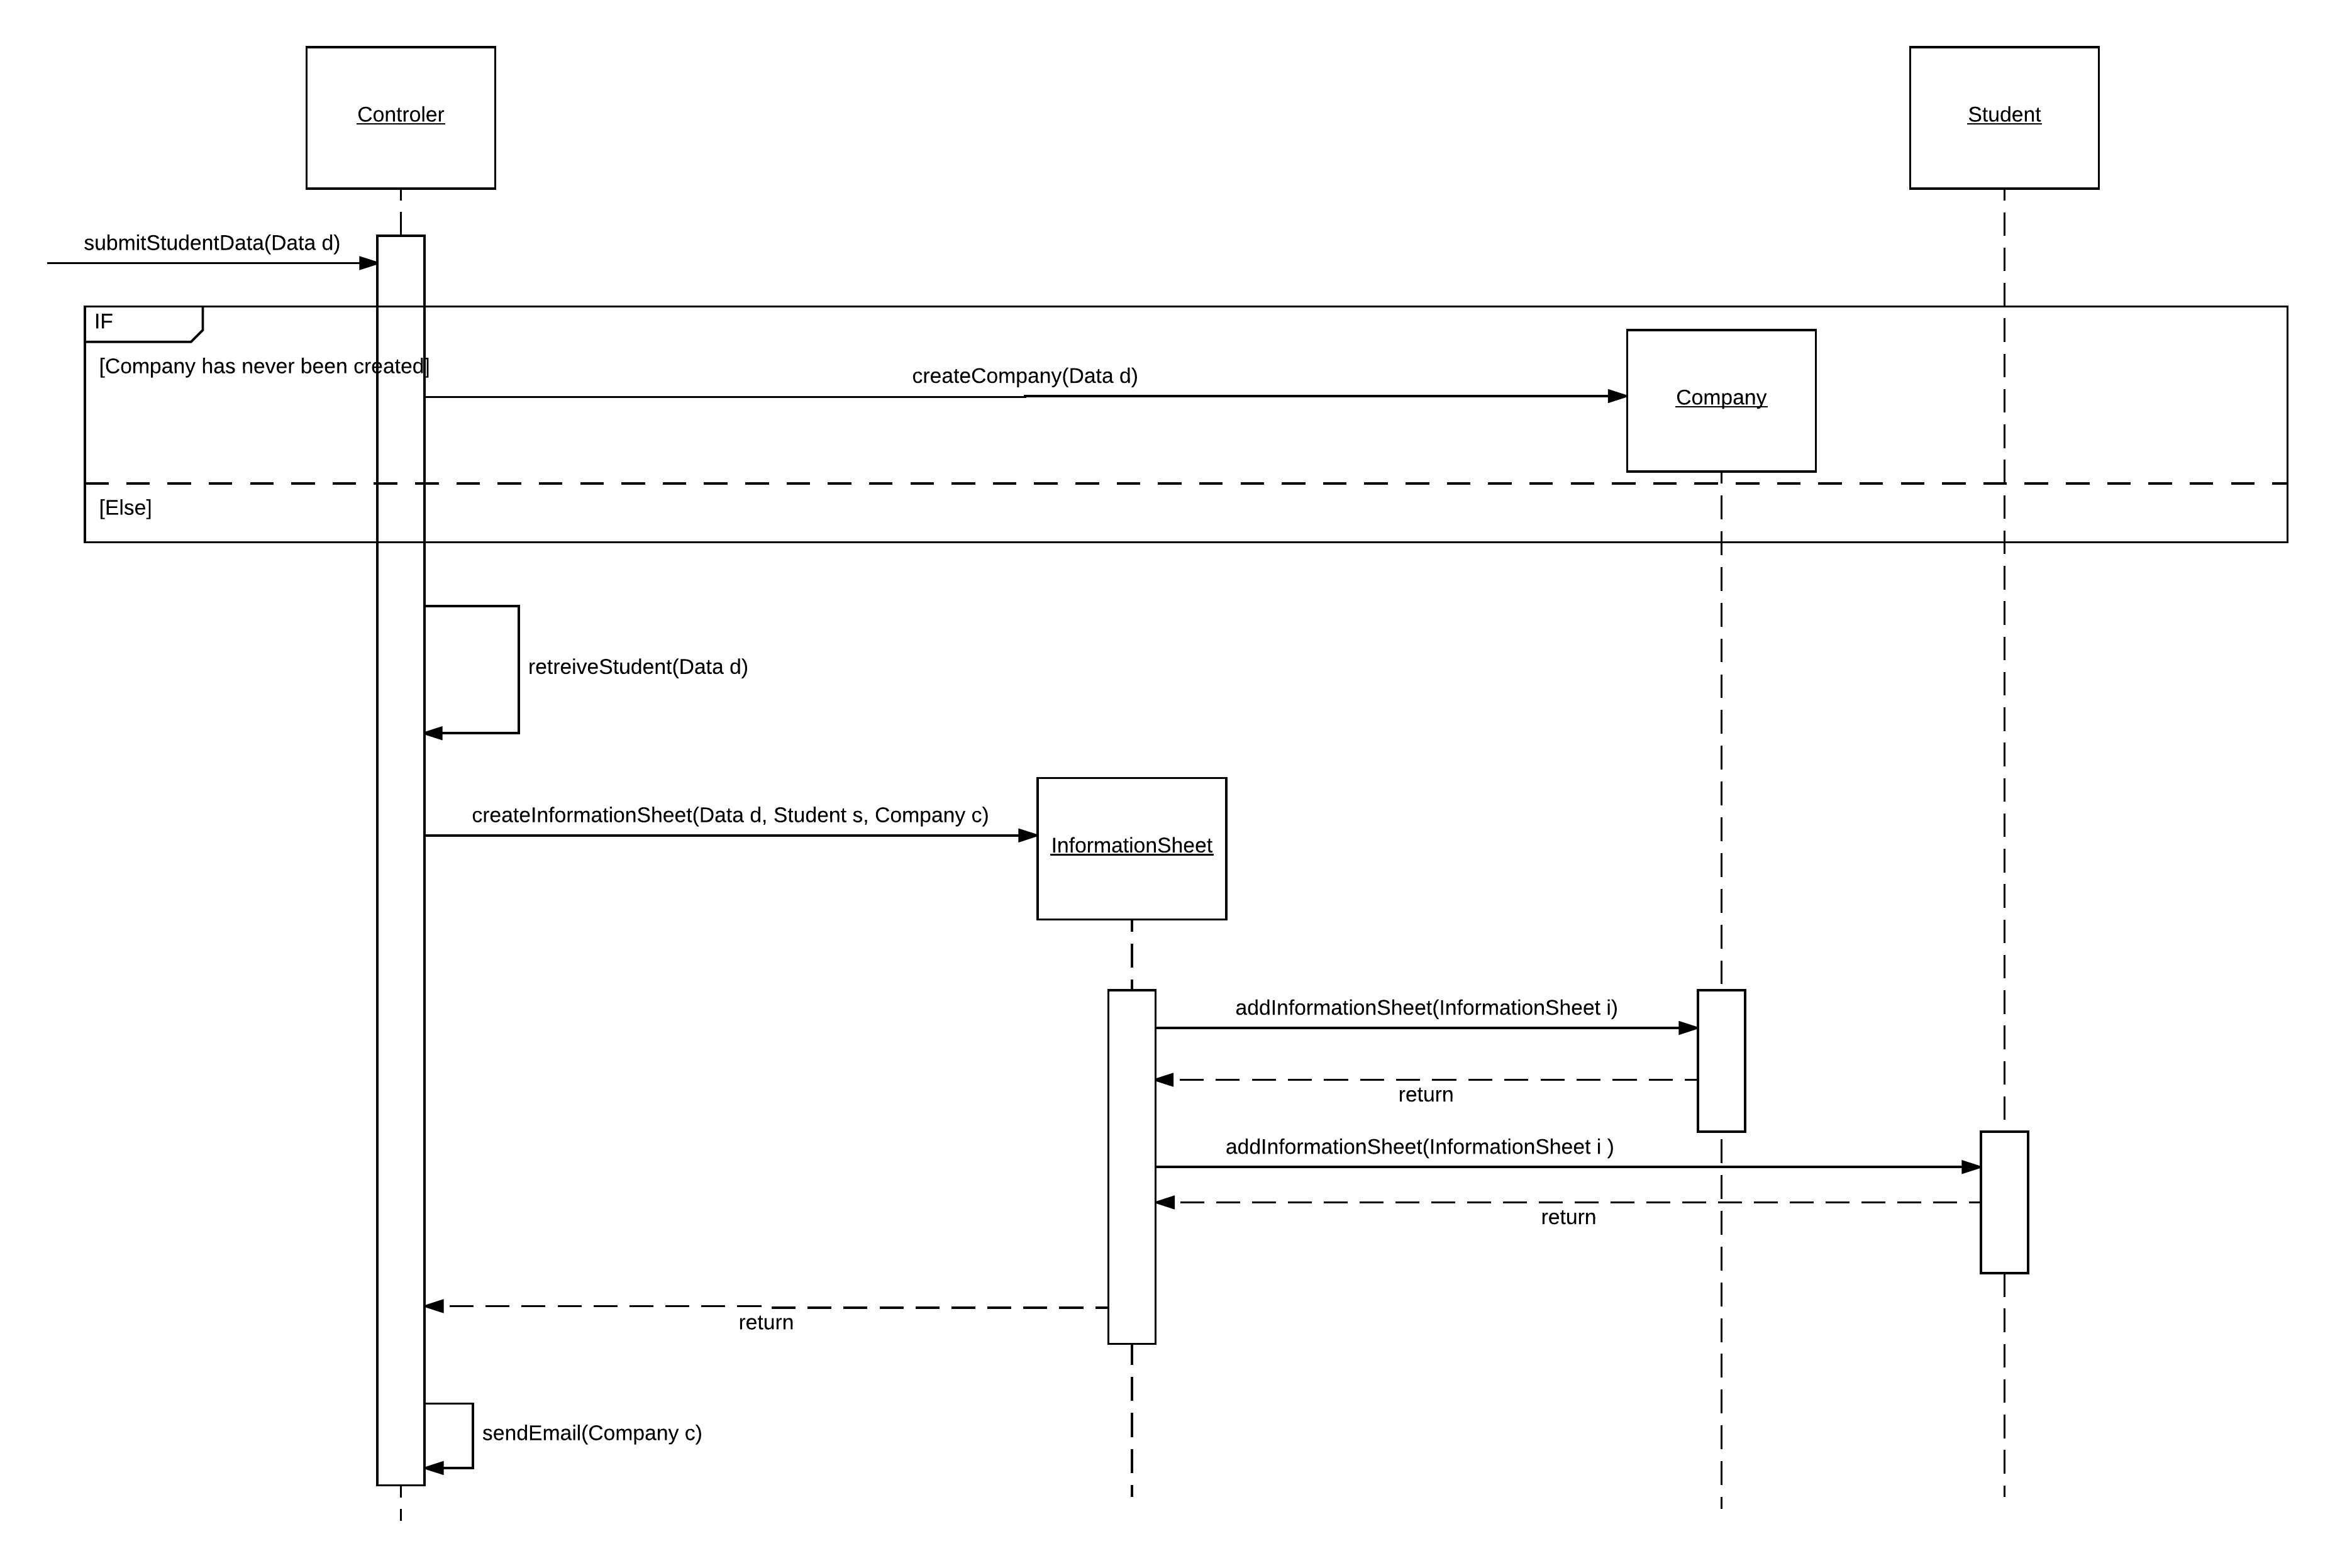
\includegraphics[width=15cm]{images/submitStudentSeqDiagram.png}
\caption{Diagramme de séquence de la saisie de la fiche de renseignement par l'étudiant}
\end{figure}

	Pour ce qui est du diagramme de séquence plus modeste, concernant la saisie de la fiche de renseignement par l'entreprise, 
la seule action réalisée est par le contrôleur lorsqu'il recoit les informations à travers la fonction "submitCompanyInformation(Data d)",
est de compléter les informations incluses dans la bonne instance de "InformationSheet".

\begin{figure}[h]
\centering
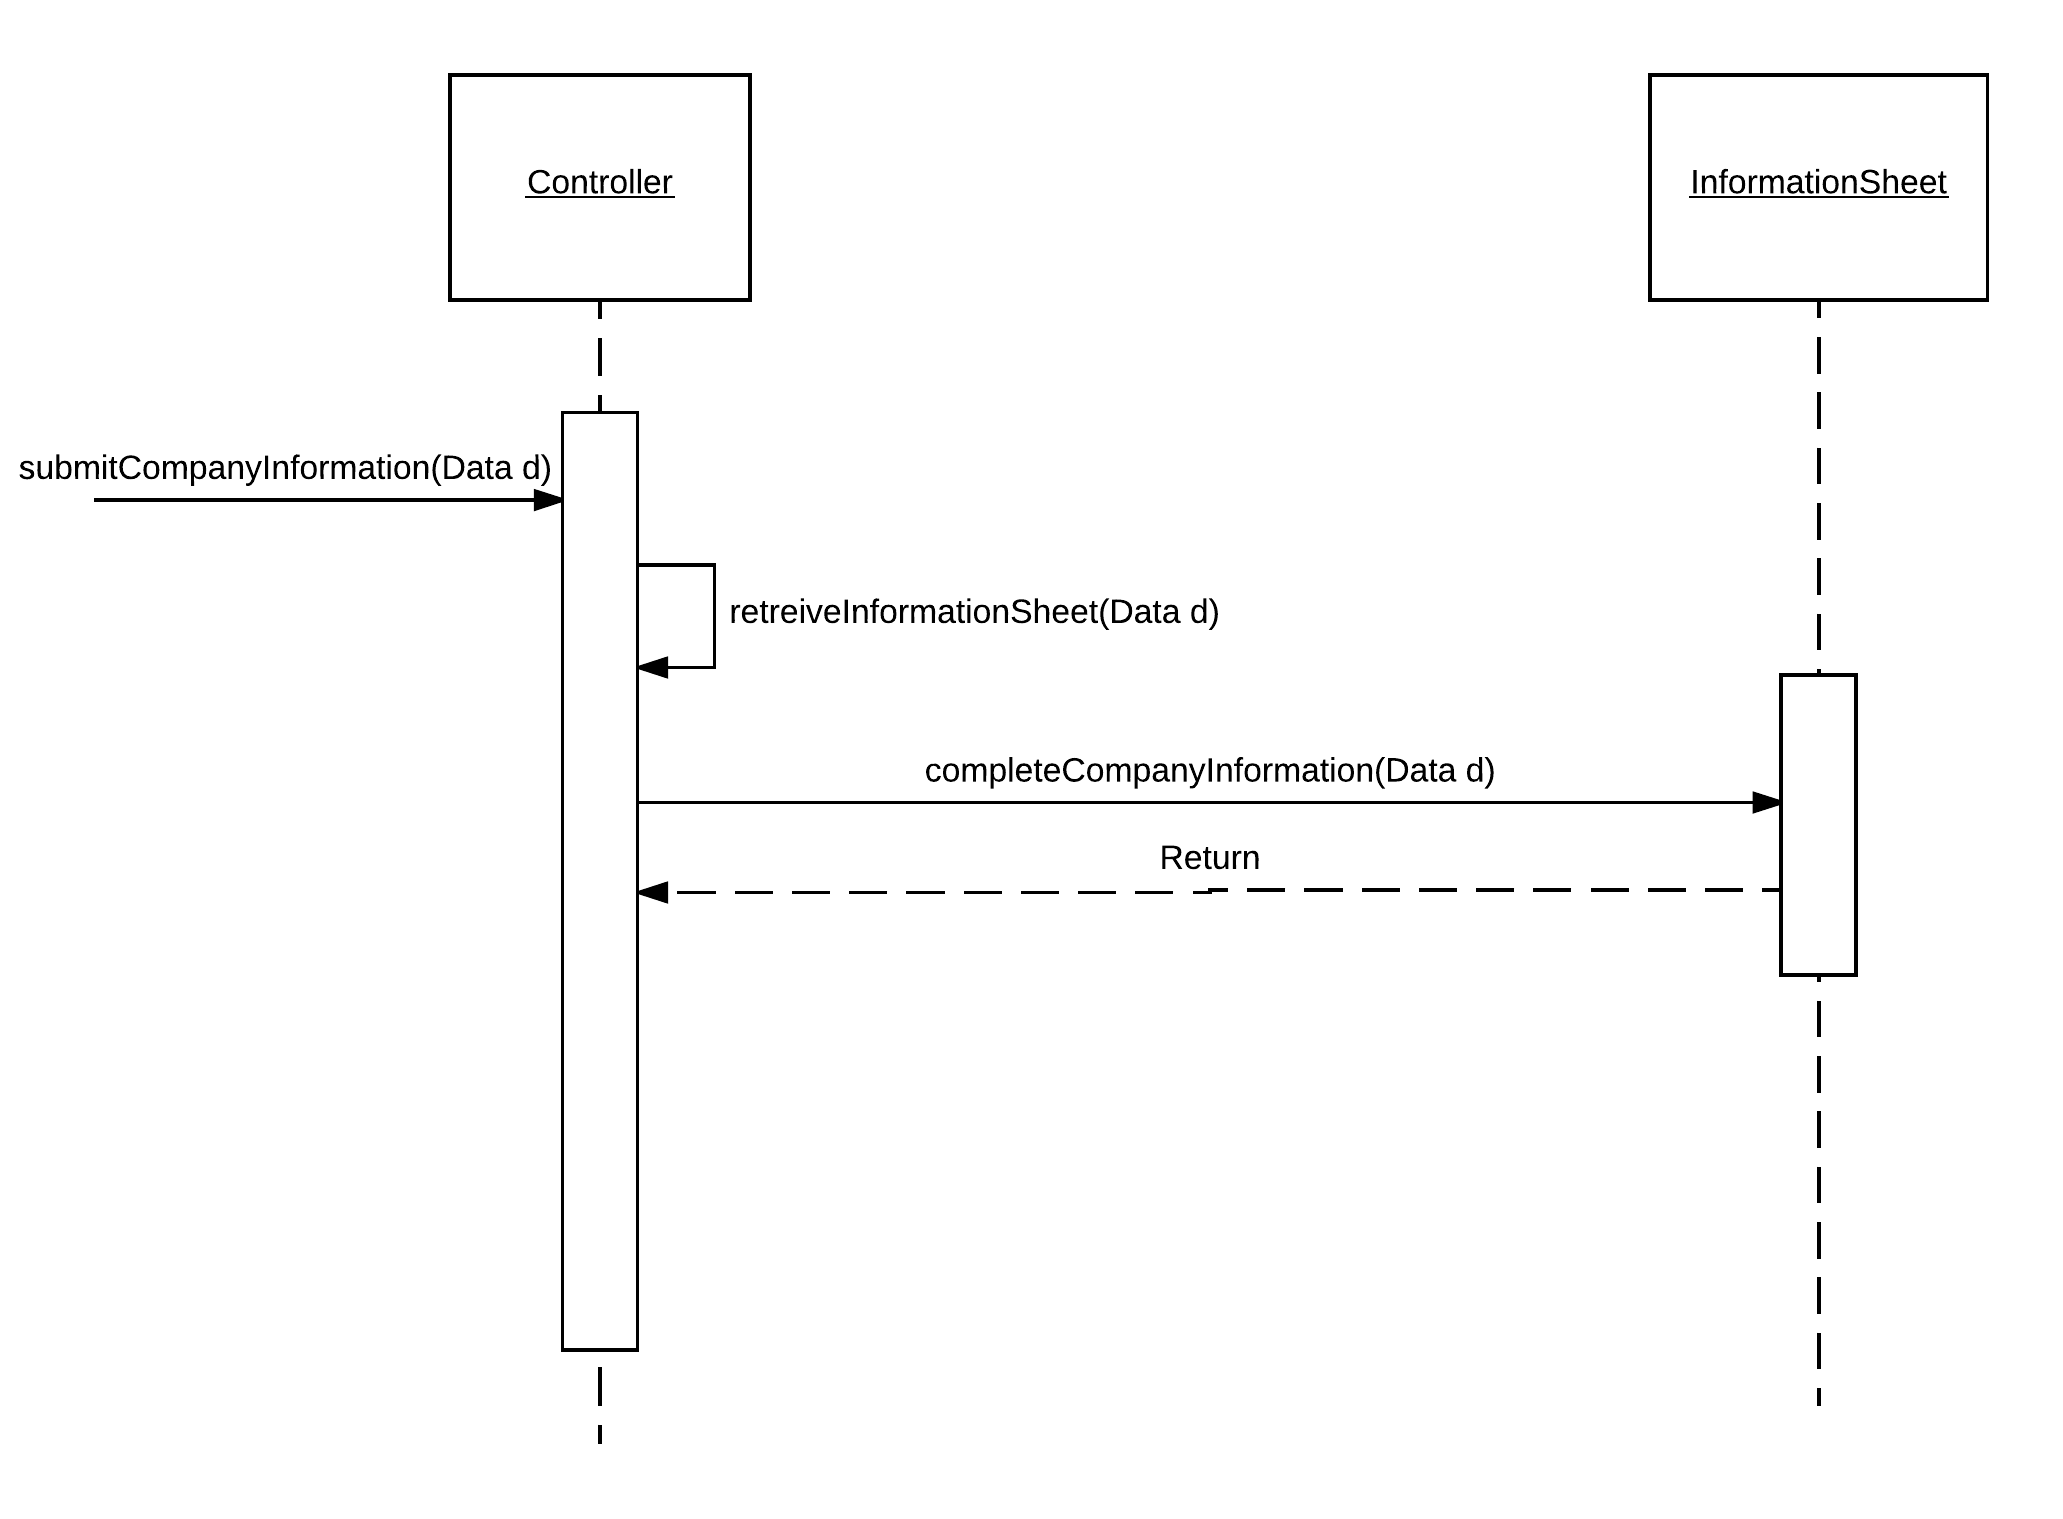
\includegraphics[width=15cm]{images/submitCompanySeqDiagram.png}
\caption{Diagramme de séquence de la saisie de la fiche de renseignement par le responsable en entreprise}
\end{figure}

\newpage
\section{Cas de la validation}

	Le diagramme de séquence représentant le cas de la validation d'une fiche de renseignement par le professeur référent, débute 
à partir du moment où la classe gérant l'interface graphique appelle la fonction "submitDecision(Data d)". On suppose ici que 
le professeur a eu les choix suivants : valider la fiche de renseignement, fiche de renseignement invalide puisque ne correspondant 
pas aux exigeances du stage ou invalide car elle est incomplète. 

	Dans le cas où la fiche est bien validée, on se propose de sauvegarder dans la bonne instance de "InformationSheet" le fait qu'elle est 
validée. Ensuite, puisqu'on est certain d'avoir une bonne version de la fiche de renseignement, on sauvegarde les informations en dur 
dans la base de donnée. Enfin, on envoie un mail ou une simple notification applicative dans le but de prévenir les principaux intéressés :
l'étudiant, le responsable en entreprise et le personnel administratif en charge de gérer les conventions de stage.

	Dans le cas où la fiche n'est pas validée et seulement à compléter, on se propose seulement de prévenir le responsable en entreprise dans 
le but qu'il puisse compléter. Cette notification pourra être accompagnée d'une remarque si le professeur référent le juge utile. 

	Dans le dernier cas, il faut réinitialiser la procédure de demande de stage. C'est dans ce but qu'on se propose de simplement supprimer 
les liens entre les bonnes instances de "Student", de "Company" et de "InformationSheet". Un mail sera envoyé dans le but d'informer l'étudiant
qu'il faudra poursuivre en trouvant un autre stage et l'entreprise pour qu'elle sache que le stage ne correspondait pas aux exigeances spécifiées
par l'école. 

\newpage
\begin{figure}[h]
\centering
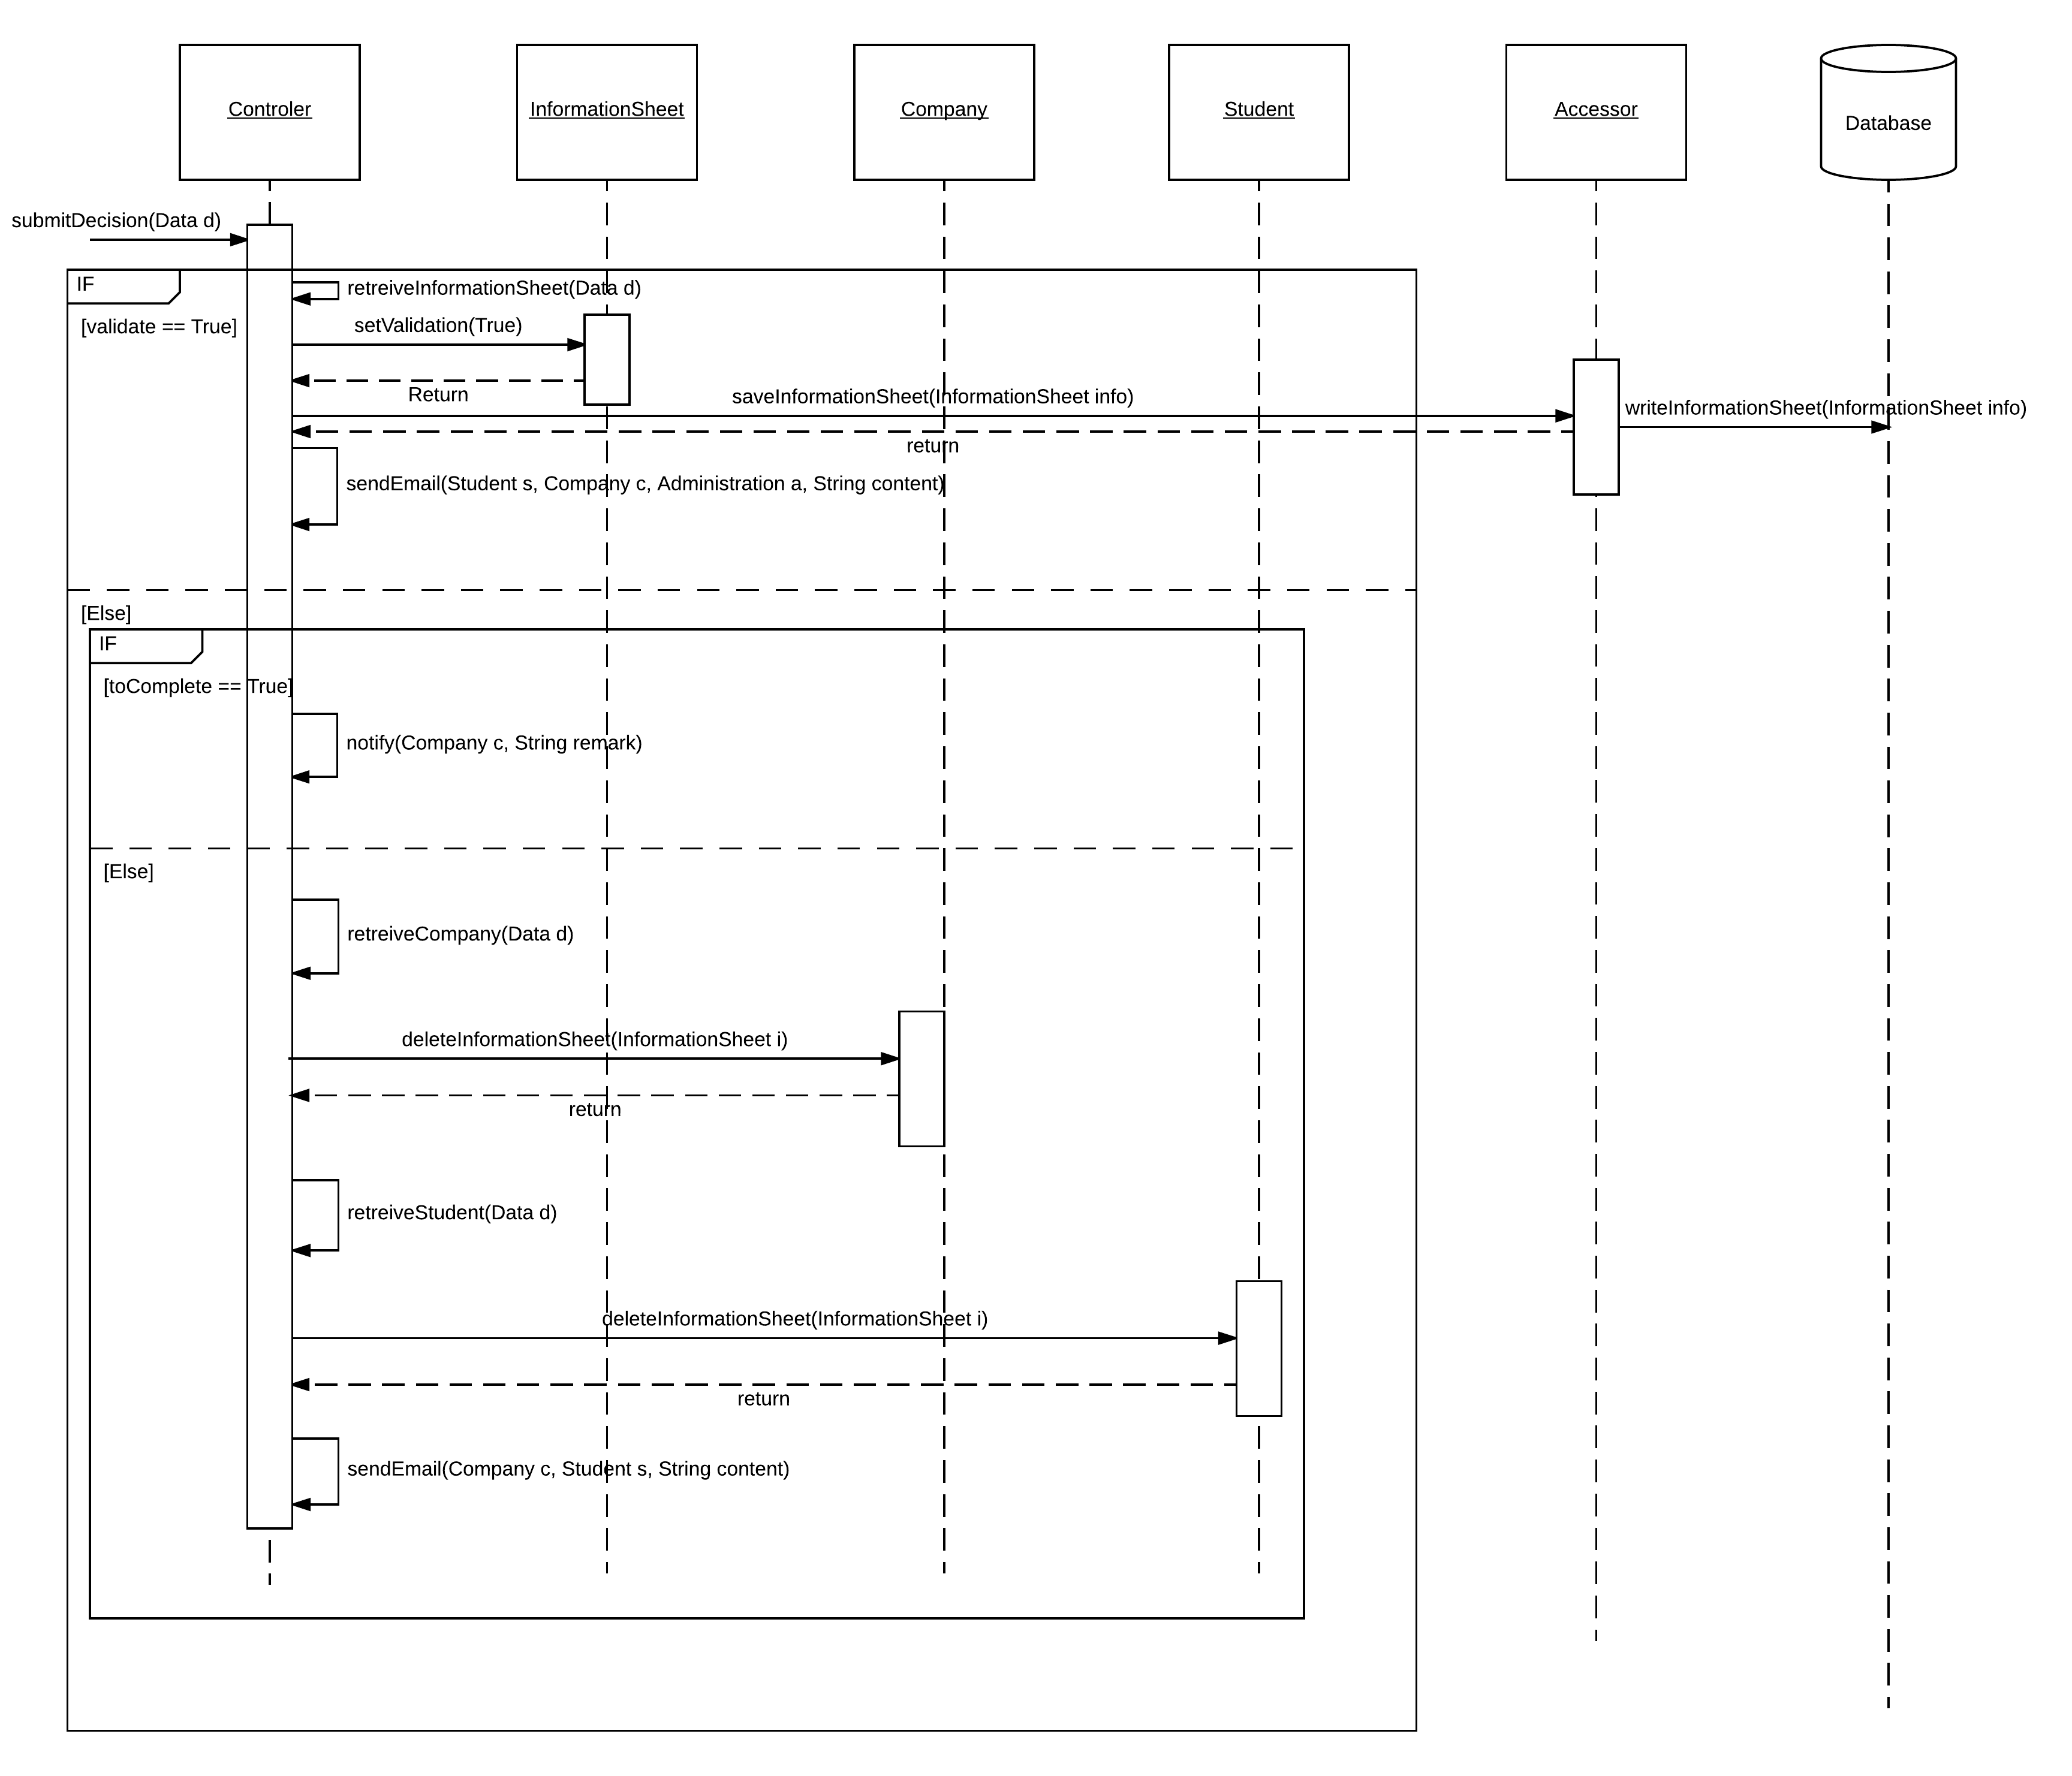
\includegraphics[width=15cm]{images/validationSeqDiagram.png}
\caption{Diagramme de séquence de la validation de la fiche de renseignement}
\end{figure}

\newpage
\section{Cas du changement d'année}

	Pour ce diagramme de séquence, on suppose que la fonction est appelée par l'utilisateur au moment où les notes des stages
précédant ont toutes été établies. Un système de deadlines sera mis en place par les professeurs à leur convenance. 

	Le diagramme de séquence représentant le cas de la transition d'une année scolaire à l'autre, débute à partir du moment
où la classe gérant l'interface graphique appelle la fonction "submisStudentStatus(Data d)". On suppose ici que les données
sont sous forme d'une table clés-valeurs. De plus, on aura la liste des nouveaux professeurs référents, ainsi que la liste des professeurs
responsable des différents stages. La première est pour le nom de l'élève et la deuxième est pour l'année dans laquelle
il passera. La procédure se répétera pour chaque élève. On commence par savoir si l'élève est nouveau en regardant sa prochaine année.
S'il est nouveau, on lui créé une instance en initialisant ses données (son année, son nom), sinon on retrouve l'instance de "Student" 
correspondant à l'élève, ce qui nous donne accès à son année courrante. 

	Si c'est un quatrième année, celà veut dire qu'on a déjà retiré ses informations de la base de donnée. Sinon, il faut retrouver 
l'entreprise où l'élève a effectué son dernier stage ainsi que l'instance de "InformationSheet" correspondant. De cette manière, on peut 
supprimer le lien entre l'instance de "Company" et l'instance de "InformationSheet" ainsi que réinitialiser les informations de 
"InformationSheet". De ce fait, si un élève d'une année passe à une nouvelle année, on peut supprimer les informations du stage précédant 
dans la base de donnée pour qu'il puisse commencer un nouveau stage. Si un élève redouble une année, on ne supprime pas son stage. Il ne 
devra ainsi pas réaliser un nouveau stage. Pour le passage de la 2ème à le 3ème année, ainsi que pour le passage de la 1ère à la 2ème année, 
on s'assure également d'attribuer à l'élève son nouveau professeur référent qui l'aidera au fur et à mesure du déroulement de son stage. 
Il n'est pas nécessaire d'attribuer de professeur référent en première année pour le stage ouvrier. 

	Enfin, indépendamment du choix des élèves, on met à jour les professeurs responsables des stages de 1A, des stages de 2A ainsi que 
des stages de 3A.  

\newpage
\begin{figure}[h]
\centering
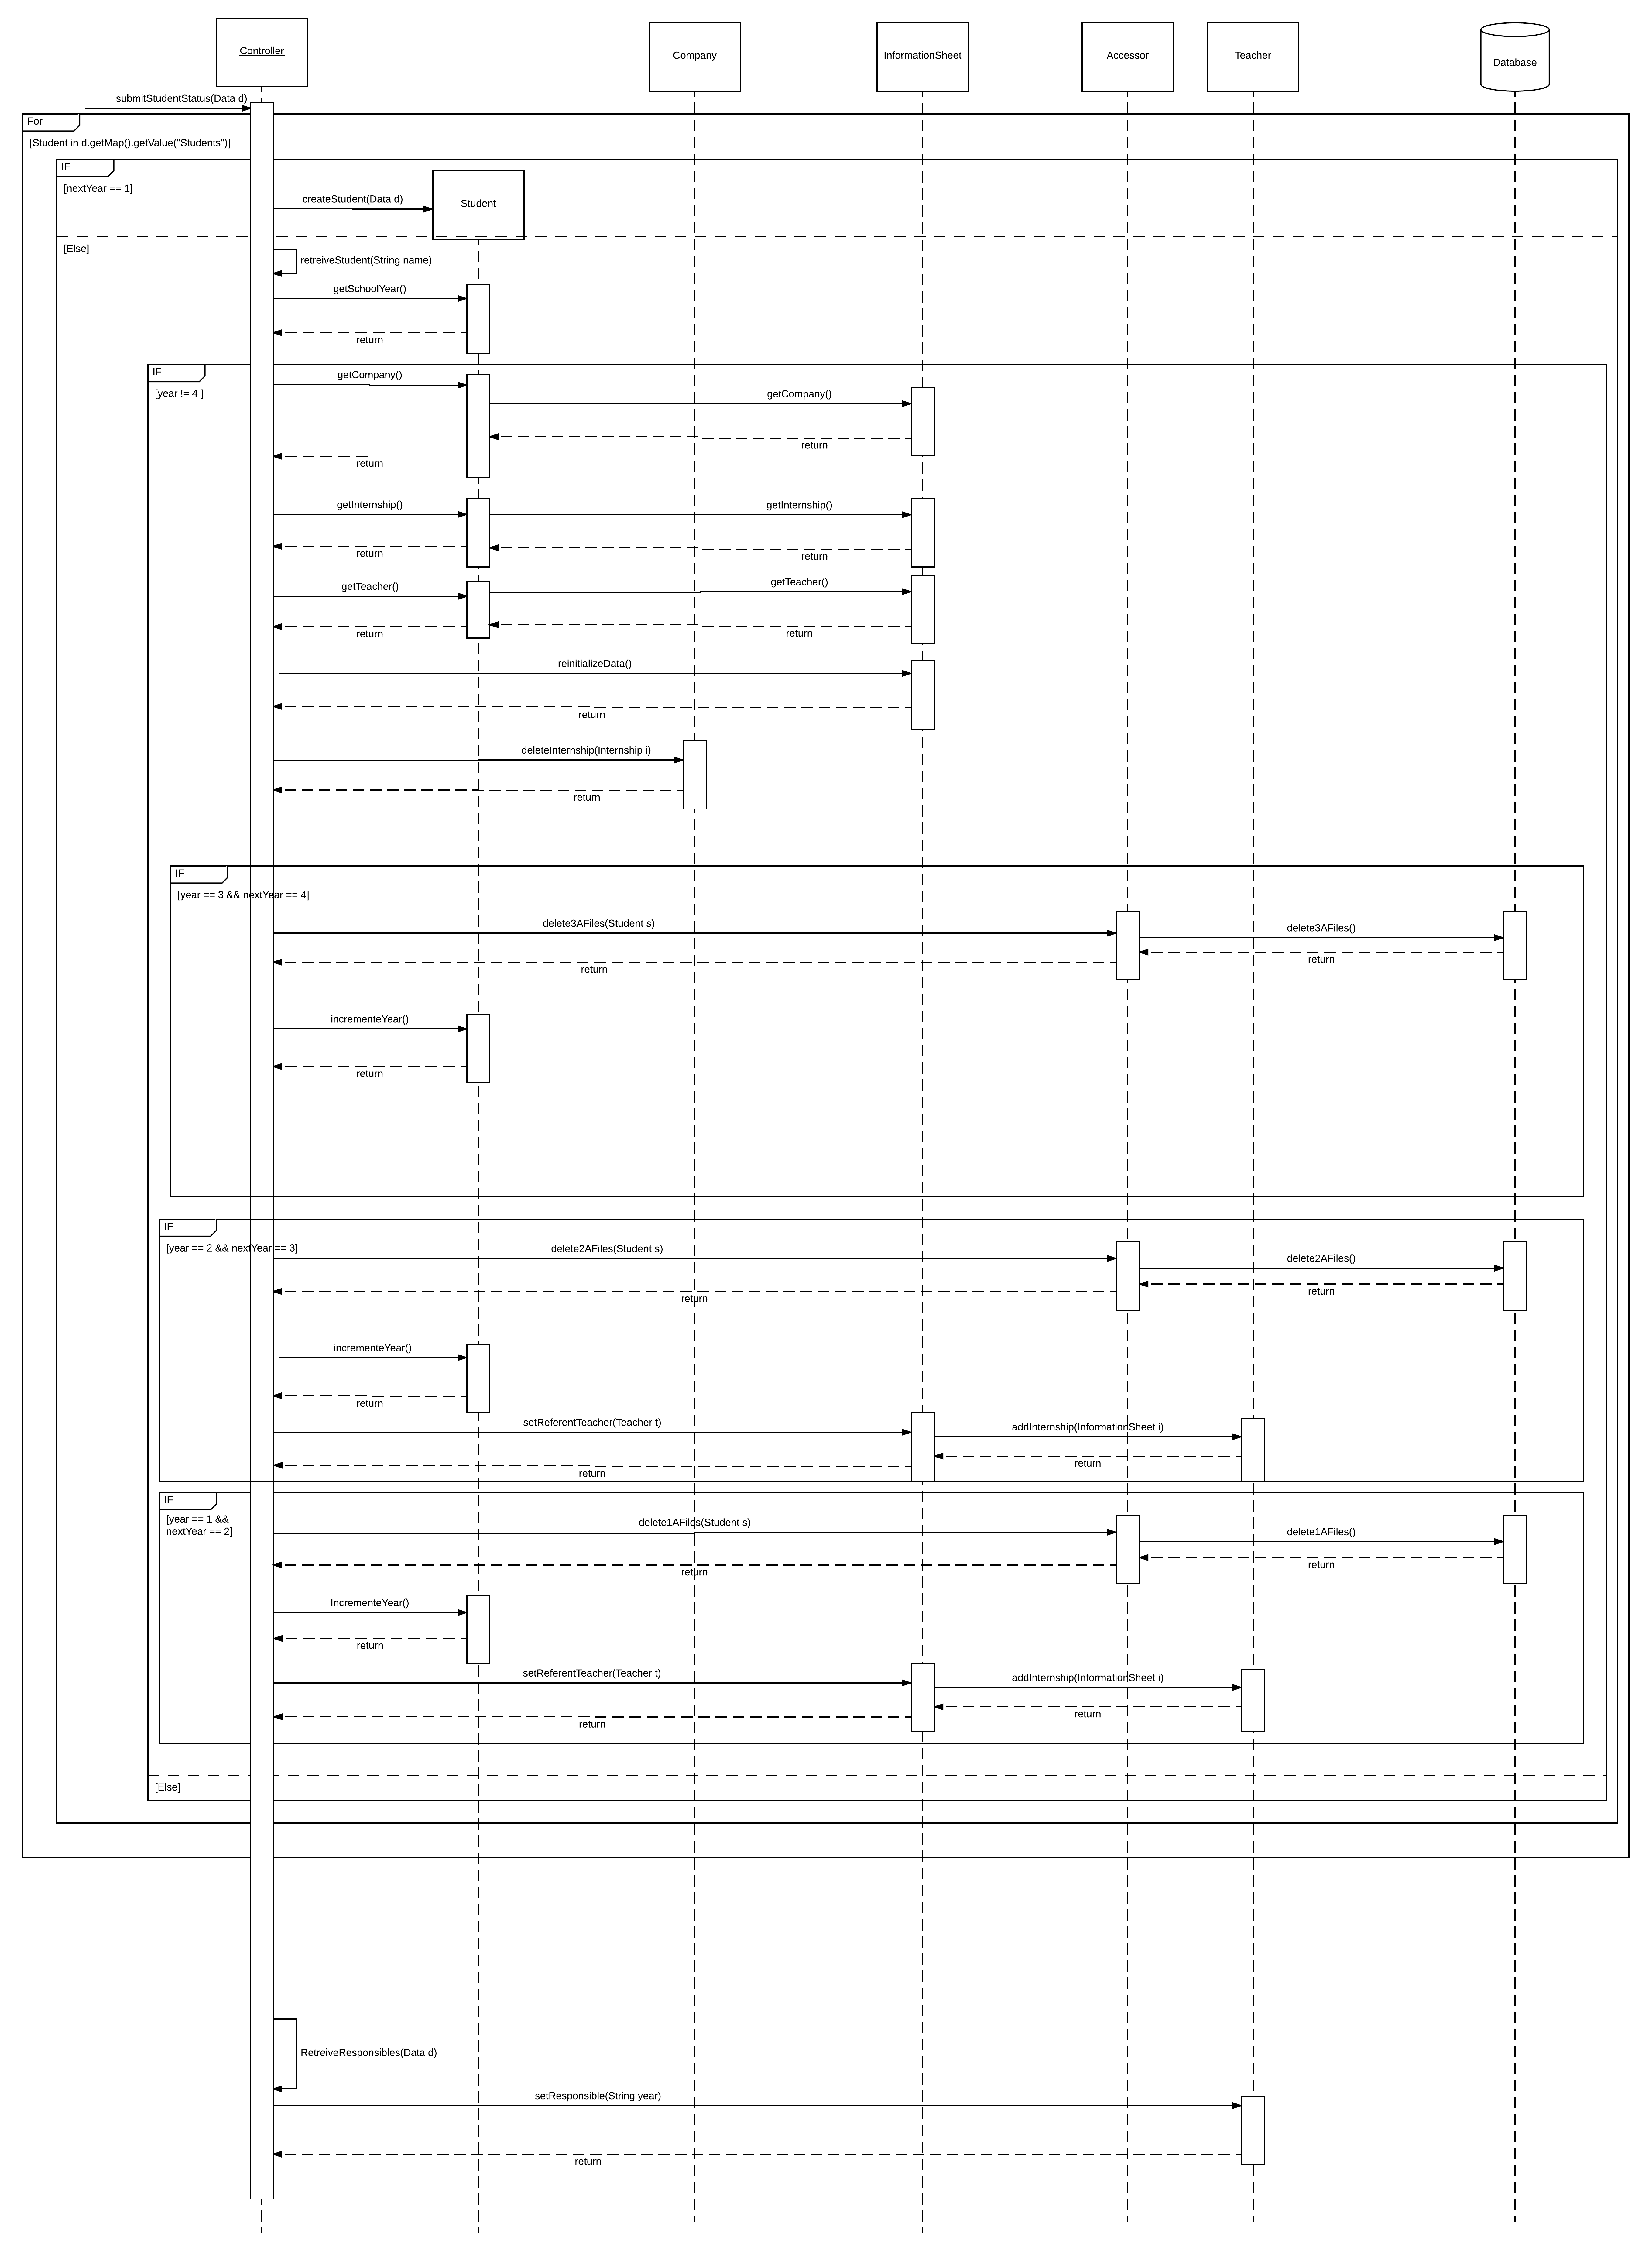
\includegraphics[width=15cm]{images/newYearSeqDiag.png}
\caption{Diagramme de séquence de la transition d'une année scolaire à l'autre}
\end{figure}

\newpage
\chapter{Diagramme de classe}
\addcontentsline{toc}{chapter}{Diagramme de classe}

Ce diagramme illustre les classes et leurs interactions entre elles. Une instance d'une classe représente un objet dynamique. Le Controller est le coeur du programme car il contient la méthode main et il va dicter l'exécution en fonction des actions des utilisateurs. Il possède un attribut Accessor dont le rôle est d'accèder, d'écrire et de supprimer dans la base de données. L'informationSheet lie un étudiant (Student), un professeur référent(Teacher) et une entreprise(Company). On remarque qu'un enseignant possède un tableau d'InformationSheet car il peut superviser plusieurs élèves. Ces acteurs héritent de la superclasse User car ils partagent des attributs comme le nom, l'id et le type d'utilisateurs. La classe Data représente les données saisies par les utilisateurs de l'application. Elle possède une HashMap de taille size. Les clés et les valeurs sont des Strings. La clé constitue le nom du champ et la valeur son contenu.Enfin, l'informationSheet possède un tableau de deux Data, celle de la partie étudiante ainsi que la partie entreprise de la fiche d'informations.

\begin{figure}[!h]
\centering
\includegraphics[width=15cm]{images/classDiagramme.png}
\caption{Diagramme de classe}
\end{figure}

\end{document}
